
\newpage 
\section{An Introduction to Programming}

\subsection{Designing computer programs}

Designing a computer program can be a complicated business. It often
requires a  great deal of creativity, a considerable understanding of
the task or process being automated, a good eye for accuracy, and
finally a large degree of patience. 

In industry, the process of designing a computer program is separated from
the task of actually writing the program itself. This is because the skills
required for each task can be quite different. 

In a professional setting, the process of program design often starts
with an idea supplied by a  
{\em customer}. The customer may telephone you
stating that they are  
considering automating the creating of a rota of workers, for example,
and that they need a program to allocate workers and email them with
their schedule. The program designer's task is then to write 
a document stating exactly what the 
customer requires, which can then be passed on to the programmers
and turned into code; this document is called the {\em program specification}. 

Writing a program specification is difficult, particularly because you 
need to pitch it at exactly the right level. A specification which states 

\begin{quote}
`Allocate time slots to workers and email them their schedules'
\end{quote}

is probably not detailed enough for a programmer to successfully write a 
piece of code which will do exactly what the customer is looking for. The
programmer may (legitimately) write some code which allocates all
hours to one worker, for example; this after all meets the
specification, though probably does not wwwork very well for the customer.

Alternatively, a specification which states

\begin{quote}
`Line 10: Assign to the worker with least hours the next time slot in
the rota, unless it is an early morning slot in which case find a
worker who has a car\ldots'
\end{quote}

may be too detailed for the programmer to have complete control over the 
implementation. The specification will probably also be extremely long and 
may, as here, contain ambiguities. 

So as you can see, writing a specification is not as straightforward as it 
first seems. Developing an appropriate program specification is an
important skill for good programming.

\subsubsection{Writing your own specifications} 

Most specifications are written either in {\em natural
language} and/or some form of {\em Mathematics} or {\em Logic}.
Natural language is perhaps the easiest way to communicate ideas, as
most of  us understand one language or another, English or Spanish for
example. If you are to  
write specifications in a natural language then you must make sure that the
specification is unambiguous. 

The closer we move towards 
maths (or logic) the less chance there is of introducing any ambiguities. 
You may learn more about using what
are known as {\em formal methods} later in your degree course.
For now, we will rely on attempting to write specifications as clearly
and as easy to read as possible. Programs and their specifications
need to be understandable by other people.

\subsection{Building computer programs}

Building a computer program is the task traditionally described
as {\em programming}. 
Despite many misconceptions, programming is rarely about sitting at a
desk littered with cans of Red Bull and bashing out some obscure lines
of instructions which reflect the programmer's thoughts and insights on a
particular problem. Programming is an exact and detailed science which
involves methodically translating {\em abstract}  
specifications
into more {\em concrete} implementations. The concrete implementation
is traditionally known as program {\em code}. 

\subsubsection{Abstract and concrete}

So what exactly is all this talk about {\em concrete} and {\em abstract}?\\


You have seen already, in the description of a specification, that when we 
describe a problem which we may want to computerise, we should choose 
carefully the level of detail at which the problem is described. 
In writing a specification 
we must not get drawn in to any nitty-gritty points which are not
wholly in the domain of the problem itself. But why do we make such a
fuss about this, and does it really matter?

Well, yes it does. When we program it is desirable to have as much freedom as 
possible: the freedom to choose a suitable programming language; choose 
our own structure and individual style; and maybe reuse bits of programs, 
to save time or money for example.

\begin{figure}
\centering
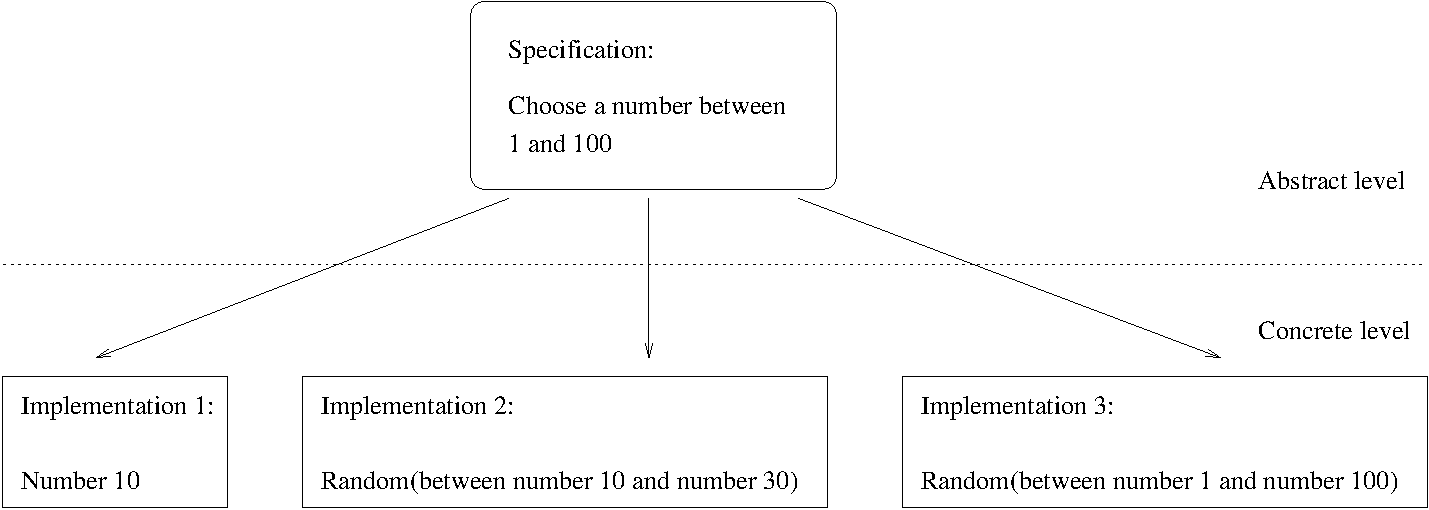
\includegraphics[width=5in]{abstract.pdf}
  \caption{\small Example of abstract- and concrete-level design 
           \label{specimp}}
\end{figure}

\noindent
In fact, it is possible to have many different programs 
which implement the same specification. Consider Figure~\ref{specimp}
for example. 
Here we have a specification which states, ``Choose a number between 1 and 
100''. There are three implementations of this specification in the figure: 

\begin{itemize}

\item
The first program simply produces the number 10. This, you may think, does
not meet the specification given, but think about it carefully. The 
specification says choose a number between 1 and 100, and the program does,
it chooses the number 10. It chooses the number 10 each time the
program is run of course, which 
is probably not what the person who wrote the specification wanted to happen.
But the specification does not say that the number chosen should be different
each time the program is run, so effectively the program is a perfectly 
good implementation of the specification. 

\item
The second program produces a random number between 10 and 30. This also 
meets the specification as the program certainly does choose a number 
between 1 and 100. Again, this is probably not what the person who wrote
the specification intended. 

\item
The third program is probably what you would have expected. It randomly chooses
a number 
between 1 and 100. This also meets the specification and had the 
specification been written more carefully, stating, ``...a different number
in this range should be chosen with equal chance each time the program is 
run...'', then this would be the only valid implementation of the 
specification written above.

\end{itemize}


This may seem a little confusing. Why is it useful to have a number of 
possible computer programs which implement a single abstract specification?
The point is
that it may not matter to the customer exactly what the program does,  
provided that it is within the bounds of the specification. Therefore, the 
programmer has flexibility when producing a program, and the customer
receives a program which meets their requirements. Everyone wins. 

Abstract specifications are useful as they allow customers who might
be requesting a software system to write a collection of unambiguous
requirements. The costumers may pass this specification to a number of different
programmers and receive a number of different programs
back. Although these programs may be different and may be written in a
number of different programming languages, on a number of different
machines, they will all act
exactly as the specification states. The specification therefore acts
as a {\em contract} between the customer and the programmer, and a
contract between the abstract description and the concrete
implementation. 


\subsubsection{Translation}

Programming is the business of taking an abstract-level specification
and translating it into a concrete-level piece of code, and, as we
have already seen,  programmers may 
do this translation in an assortment of different ways. 
Just as it is important to carefully write a specification, it is also 
important to make sure that the program implementation is an accurate
coding of the description in the specification.


The translation between an abstract-level specification and a concrete-level
design is technically called a {\em refinement}. Each of the programs
in Figure~\ref{specimp} is a valid refinement of the specification.


Usually a specification will have a number of complicated clauses, and 
may also span a number of pages. Although the specification 
may be exact in its description, a programmer may make a mistake 
when reading it and consequently code something different. For this 
reason, some specification methods have complicated mathematical rules 
which translate a piece of the specification (usually written mathematically)
into the corresponding piece of program code. These rules are 
known as {\em refinement rules}. 

\subsection{Testing computer programs}

Testing a computer program is an extremely important business. There are many
well-known examples cite where software has failed due to inadequate testing.
One such example is the case ofthe  Ariane 5 launch vehicle.
In the thrust direction control unit, 
code was reused from Ariane 4.
In this code, horizontal speed was represented
by a 16-bit value.
But horizontal speed in Ariane 5 was greater,
and caused an overflow, which raised an exception.
The specification said (very foolishly) that
if an exception arose, the processor should be 
shut down and restarted.
Shutting the processor down caused the thrust
direction to jump suddenly sideways, which
broke the rocket in half \ldots It can be argued that more extensive
and methodical testing could have avoided this accident.


Of course not every example of software failure will end in a disaster 
quite as catastrophic as this. However, the consequences of  code failure
may prove to have just as much of an impact on the results of a small company,
or on the grade assigned to your computing assignment, for example.

{\em Failure} is defined as the 
departure of the behaviour of a program from its requirements. Unfortunately,
it is not possible to show the absence of failure by testing, as testing 
will only tell us whether a program fails in a particular scenario or not.
The purpose of testing is to eliminate as many problems in the code as 
possible. This  
increases the programmer's (and user's) confidence in the piece of code. As
the number of failures detected in a program becomes less, the more you will 
feel that the program exhibits the correct behaviour.      

\subsubsection{Methods of testing}

The experimental science of software testing has been the subject of research
for a number of years. Consequently, there are a number of testing methods
which are shown to be effective. We will see, and use, a few of these methods
in this course. 

\paragraph{Test of logical paths of program} One useful way to test a
program is to examine all the logical paths. Consider this example:

\begin{minted}{java}
   while (x < 10) {
       if (even(x)) {
           System.out.println("The number is even\n");
        } else {
           System.out.println("The number is odd\n");
           x = x + 1;
       }
   }
\end{minted}

To test the logical paths of this short piece of code the user would need 
to design tests to cover at least three cases: The case when \javaIn{x} is 
greater than or equal to 10, in which case the while loop would not be
executed at all; the case when \javaIn{x} is less than 10 and is even, in which 
case you would expect `{\tt The number is even}' to be printed at least once, 
and finally the test when \javaIn{x} is less than 10 and is odd, in which case 
you would expect `{\tt The number is odd}' to be printed at least once.


Forgetting one of these cases would mean that you have not tested part of the 
code; this may be the piece of code which blows up, or
wipes the hard disk, or \ldots Would you expect any of the logical paths
in the program to reveal an error in the above code?

\paragraph{Range of inputs} Another way to test the example program
would be to test the range of  
inputs. If we can be sure that the program produces the right output for
each valid (and even invalid) input, then we can be a bit more sure that it
does what we expect. We may for example have tested the program with a 
negative value, a positive value and the value 0.

\noindent
Boundary cases are also important. You may want to check that the computer
deals correctly with the highest possible number and the lowest possible 
number. Finally, you may want to put some spurious values into the program:
what happens when you type in a character, for example, or if you just press 
the `Enter' key, or if you just sit on the keyboard?

\noindent
Of course you have to select your range of inputs carefully. Selecting the 
numbers \javaIn{137645813451875},  
\javaIn{0.14643528745}, \javaIn{-23} and \javaIn{19}, say, 
would not have found the infinite loop in the program.

\paragraph{Systematic tests} It is all very well to test the logical
paths of the program and 
the ranges of input, but it is sometimes the sequence of operations in
a program which causes it to break. For example, in the case of an
airplane the `landing-gear down' and
`increase throttle' routines may both work exceptionally well by themselves, 
but putting the landing-gear down and then increasing the throttle may cause
the plane to head towards the ground at a rapid speed. This is probably not
what you want!


It may be worth testing a sequence of operations in your program, testing
all the permutations of the routines 
to make sure that one specific ordering does not exhibit any
unexpected behaviour.  

\paragraph{Random tests} Random testing is a perfectly legitimate
activity, but do not expect it to consistently come up with all the
errors which may be detected by a logical or systematic approach.

A true random test of a program is actually quite difficult to 
achieve. It would probably require a random number generator to 
choose between the routines in the program which were to be  
tested. A random test would also require a similar random 
selection activity to choose random input data to the program;
of course the amount of data itself must also be randomly chosen.
So be careful when you use the term `random testing'.
 
\paragraph{Intuitive tests} The process that people often think of as
random testing is actually called {\it intuitive testing}.  

After you have spent some time programming you may become aware of common
errors which appear in programs. A program that stores and deletes a 
collection of names will often fail if the first thing you ask it to 
do is to delete. Programs which accept characters as input will often
break  if you feed in a `Control' character (which is a special
character that cannot be printed 
to screen).

Choosing cases like this to test your program is not a random 
activity, as you are usually selecting the tests based on your 
intuition as a programmer. So when you run a program for the 
first time and select a number of seemingly random operations, 
you will probably find yourself going through a number of cases
which you expect to work, followed by one or two cases in which 
you think the program may break. 

These tests usually require a bit of 
thought, but you can come up with some interesting results quite quickly. 
 

\paragraph{Test application} This consists of
software that runs alongside the program to be tested. The test
application, also known as a test rig, may  generate test data, supply
tests, and record and 
calibrate the  results as the testing takes place.

Test applications are useful as they automate  
the testing process, removing any possibility of human error.
They also allow a large number of tests to be carried out 
automatically; you may for example run the test application overnight,
checking the  results the following morning.  

Test rigs also allow large systems to be tested with relative
ease. Programmers of large systems, those used by banks for example,
often use test rigs  
when they are modifying the system. This means that the results before
and after  the modification can be compared to make sure that the
system is still  operating correctly. 

One thing which is slightly ironic about test rigs is that they
themselves need testing, perhaps with test rigs, which
themselves\ldots There are software tools that allow test rigs to be
generated semi-automatically.

~

You will be encouraged to try some of these test methods during your
software development assignments, and to explain how you have tested
your software,
The method of testing you use will often be dictated by a number of factors. 
You may not have time to carry out a logical or systematic test and an
intuitive test will have to do; it may be essential that you identify
as many errors as  
possible, in which case random and range testing might not be good enough. It 
is up to you as a programmer to weigh up these factors to determine which 
method is appropriate given the situation. 
 
